\documentclass{standalone}
\usepackage{mintikz}
\usepackage{mathtools}

\begin{document}
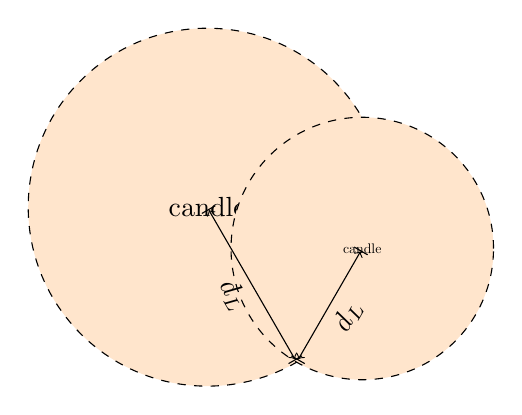
\begin{tikzpicture}[]
    \def\r{2.5}
    \coordinate (C2) at (120:\r/1.1);
    \filldraw[dashed, fill=orange!20] (C2) circle (\r/1.1);
    \node[scale=1] (candle2) at (C2) {\twemoji{candle}};
    \coordinate (C1) at (60:\r/1.5);
    \filldraw[dashed, fill=orange!20] (C1) circle (\r/1.5);
    \node[scale=.5] (candle1) at (C1) {\twemoji{candle}};
    \oeil[shift={(0, 0)}, rotate=60, scale=.5];
    \oeil[shift={(0, 0)}, rotate=120, scale=.5];
    % Grandeurs
    \node[inner sep=0] (Og) at (0,0) {};
    \node[inner sep=0] (Rg) at (candle1.center) {};
    \draw[|<->|] (Og) --
    node[below, midway, sloped]
    {$d_L$} (Rg);
    \node[inner sep=0] (Og) at (0,0) {};
    \node[inner sep=0] (Rg) at (candle2.center) {};
    \draw[|<->|] (Og) --
    node[below, midway, sloped]
    {$d_L$} (Rg);
\end{tikzpicture}
\end{document}
